\documentclass[12pt]{article}  % Specify the document class

% Commonly used packages
\usepackage[utf8]{inputenc}
\usepackage[T1]{fontenc}
\usepackage[margin=1in]{geometry}
\usepackage{amsmath}
\usepackage{graphicx}
\usepackage[
    style=ieee,
    urldate=comp,
    maxbibnames=99,
    minbibnames=99,
    maxcitenames=2,
    mincitenames=1,
    sorting=none,
    backend=biber,
    giveninits=true,
    doi=false,
    isbn=false,
    url=true,
    eprint=false
]{biblatex}
\usepackage{hyperref}  % Load hyperref last
\usepackage{tikz}
\usetikzlibrary{trees, shapes, arrows}

% Bibliography customization
\renewcommand*{\bibfont}{\small}
\setlength{\bibitemsep}{0.5\baselineskip}
\DeclareFieldFormat{url}{\url{#1}}
\DeclareFieldFormat{urldate}{\mkbibparens{accessed #1}}

% Bibliography setup
\addbibresource{references.bib}

% Document information
\title{Making Tools}
\author{Edvin T. Berhane}
\date{\today}

\begin{document}

\section*{Making Tools}

\begin{figure}
    \centering
    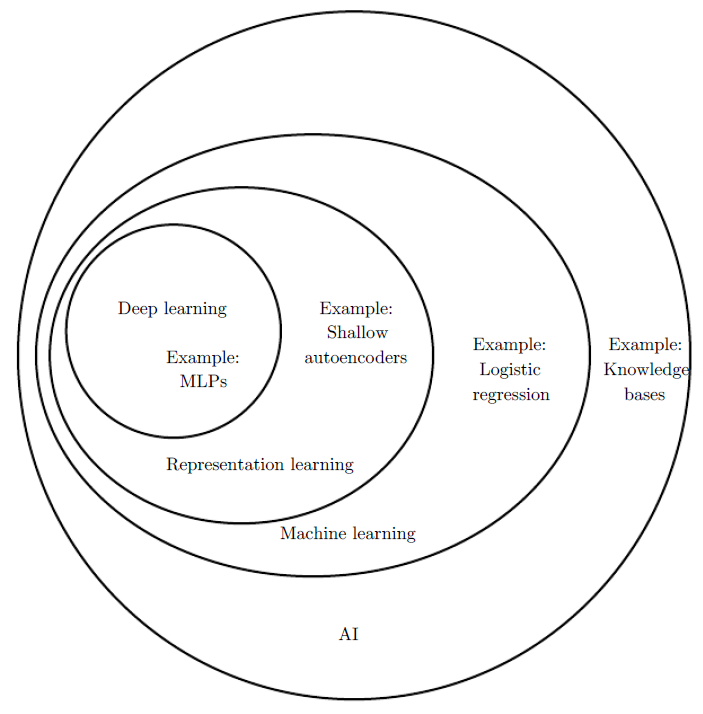
\includegraphics[width=0.5\textwidth]{figures/ai_hierarchy.png}
    \caption{Hierarchy of AI systems. Adapted from \cite{goodfellow2016deep}}
    \label{fig:ai_hierarchy_v1}
\end{figure}

\begin{figure}[h]
    \centering
    \begin{tikzpicture}[
        level distance=1.5cm,
        level 1/.style={sibling distance=4cm},
        level 2/.style={sibling distance=4cm},
        level 3/.style={sibling distance=2cm},
        every node/.style={draw=none, align=center}
    ]
        \node {Artificla Intelligence}
            child {
                node {Patterns from Data\\(Machine Learning)}
                child {
                    node {Parametrized\\representation}
                    child {
                        node {Deep Learning}
                    }
                }
                child {
                    node {Fixed\\representation}
                }
            }
            child {
                node {Symbols and Rules\\(Symbolic AI)}
            };
    \end{tikzpicture}
    \caption{Hierarchy of AI systems. Adapted from \cite{goodfellow2016deep}}
    \label{fig:ai_hierarchy}
\end{figure}

The figure \ref{fig:ai_hierarchy} illustrates the hierarchy of AI systems, from simple tools to more complex intelligent systems. This hierarchy helps us understand the progression from basic tools to advanced AI, and how different levels of complexity and autonomy define various types of systems.

\printbibliography

Questions: What makes something a "tool" vs a "system"? What makes something a "system" vs. an "intelligent system"? What makes something an artificially intelligent system? Why are some problems we want to solve in the realm of "AI" and others not? What distinction makes sense to draw? What is a "machine", "system", "tool"? Many tools have as their main purpose the creation of other tools. Think SaaS product or litography machines. 

Methods for achieving our desires. Tools enable those methods. For simplicity, we'll consider desires as fixed, even though they are in reality shaped by the societies which aim to fulfill them.

\end{document}
